\chapter{Scelte tecniche e introduzione agli esperimenti}


\section{Struttura della rete e addestramento}
\begin{flushleft}
    

La rete neurale implementata è una \textit{Multi-Layer Perceptron (MLP)} costruita utilizzando il framework PyTorch.  
La struttura definita è la seguente:
\begin{itemize}
    \item uno \textbf{strato di input} composto da 784 neuroni, corrispondenti ai pixel dell'immagine MNIST ($28 \times 28$) trasformata in un vettore unidimensionale;
    \item uno \textbf{strato nascosto} da 512 neuroni, seguito da una funzione di attivazione \textit{ReLU};
    \item un secondo \textbf{strato nascosto} da 256 neuroni, anch'esso seguito da \textit{ReLU};
    \item uno \textbf{strato di output} da 10 neuroni, che rappresentano le dieci classi del dataset MNIST (cifre da 0 a 9). In uscita viene utilizzata una funzione \textit{softmax}, che assegna ad ogni classe una probabilità di appartenenza.
\end{itemize}

La scelta della funzione di attivazione \textit{ReLU} nei layer nascosti si è rivelata vantaggiosa rispetto all’uso della funzione sigmoidea, in quanto ha consentito una convergenza più rapida e stabile del modello.  
La funzione di perdita adottata è la \textbf{Cross Entropy Loss}, particolarmente adatta ai problemi di classificazione multiclasse.  

L’ottimizzazione dei parametri è stata eseguita mediante \textbf{Stochastic Gradient Descent con Momentum (SGDM)}, il quale estende il classico metodo SGD introducendo un termine di “inerzia” che accumula le informazioni dei gradienti precedenti. La formulazione è la seguente:

\begin{equation}
\begin{aligned}
v_t &= \mu v_{t-1} - \eta \nabla_{\theta} J(\theta_t) \\
\theta_{t+1} &= \theta_t + v_t
\end{aligned}
\end{equation}

dove $\eta$ è il \textit{learning rate}, $\mu$ il coefficiente di \textit{momentum}, $J$ la funzione di costo e $\theta_t$ i parametri al tempo $t$.
\end{flushleft}

\section{Architettura di calcolo}
\begin{flushleft}
    L'architettura di calcolo utilzzata per questa tesi è molto poco potente, in particolare si tratta di un laptop HP con le seguenit specifiche:
    \begin{itemize}
        \item Numero core CPU: 4 (8 thread con Hyper-Threading)
        \item Quantità RAM: 16GB
    \end{itemize}
\end{flushleft}

\section{Introduzione agli esperimenti}
\begin{flushleft}
    
In questa sezione viene presentata la metodologia sperimentale adottata nel corso della tesi, seguendo un approccio progressivo che parte dall'implementazione di tecniche di ottimizzazione tradizionali, come l'addestramento tramite \textit{Stochastic Gradient Descent with Momentum} (SGDM) e \textit{ADAM}, per poi analizzare diverse metodologie di allenamento basate su algoritmi genetici (GA), fino alla proposta di approcci ibridi che combinano i vantaggi di entrambe le tecniche.

La presente sezione si focalizza esclusivamente sulla descrizione teorica e metodologica degli esperimenti condotti, illustrando le procedure implementate e la logica sottostante alle scelte sperimentali. I risultati numerici e l'analisi quantitativa dei dati ottenuti saranno presentati nel capitolo successivo, dove verranno supportati da tabelle comparative e rappresentazioni grafiche.

La separazione tra la componente metodologica e quella dei risultati è stata adottata per garantire maggiore chiarezza espositiva e facilitare la comprensione dell'approccio sperimentale seguito.
\end{flushleft}

\section{Allenamento con SGDM}
\begin{flushleft}
    I primi esperimenti sono stati quelli di allenare la rete con SGDM, il quale ha portato a risultati ottimali e in breve tempo. Con
    l'utilizzo di tutto il dataset (ricordiamo essere composto da 60.000 immagini) si è riusciti, analizzando vari tentativi, a raggiungere circa il 98\% di accuracy.
    Altri test, sempre con il metodo SGDM, sono stati fatti prendendo quella che è una partizione molto più piccola del dataset; questo è stato fatto per evidenziare
    i limiti di SGDM in presenza di pochi dati di training, e anche perché, come sarà spiegato, i GA, vista la potenza di calcolo a disposizione, non possono essere 
    allenati con tutto il dataset. Quindi, per fare un confronto di performance sensato, si è deciso di confrontare i due metodi a parità di dati di training.
\end{flushleft}


\begin{flushleft}
\section{Allenamento con GA non parallelizzato}
\subsection{Introduzione}
Per ragioni di efficienza computazionale , è stata presa la decisione di addestrare la rete neurale utilizzando un sottoinsieme di 1.000 istanze estratte dalle 60.000 disponibili nel dataset MNIST. Questa scelta è stata motivata dalla necessità di ridurre il carico computazionale associato all'addestramento mediante algoritmi genetici, che richiedono l'elaborazione di un numero significativamente elevato di reti neurali in parallelo.

È opportuno sottolineare che il funzionamento dell'algoritmo genetico si basa sul calcolo della funzione di \textit{fitness} per ciascun individuo della popolazione, valutando le prestazioni della rete neurale in base ai parametri specifici di ogni singolo esemplare. Per gli esperimenti condotti sono stati mantenuti costanti i seguenti iperparametri:

\begin{itemize}
    \item Dimensione della popolazione: 100 individui
    \item Numero di generazioni: 250
    \item Numero di individui \textit{elite}: 18
    \item Probabilità di \textit{crossover}: 0,6
    \item Probabilità di mutazione: 0,2
\end{itemize}

Dall'analisi dei requisiti computazionali emerge chiaramente che per ogni generazione è necessario eseguire il \textit{forward pass} su 100 reti neurali distinte, comportando un costo computazionale estremamente elevato sia in termini temporali che di utilizzo della memoria. Utilizzando partizioni di dataset più grandi di quella utilizzata (1.000 istanze), il tempo richiesto per completare l'addestramento risulterebbe proibitivo, rendendo impraticabile l'esecuzione degli esperimenti in un arco di tempo ragionevole. 

Per questa ragione, limitatamente agli esperimenti preliminari di addestramento puramente basato su algoritmi genetici, è stata adottata la strategia di utilizzare un campione significativamente ridotto rispetto alla totalità dei dati disponibili.

\subsection{Esperimenti}

Gli esperimenti sono stati condotti mantenendo fissi i parametri di mutazione e gli iperparametri precedentemente specificati, variando esclusivamente la metodologia di \textit{crossover} implementata. In particolare, sono stati analizzati i seguenti approcci:

\begin{itemize}
    \item \textit{Blend Crossover}
    \item \textit{Simulated Binary Crossover}
    \item \textit{Arithmetic Crossover}
    \item Approccio ibrido, caratterizzato dall'alternanza dei metodi sopra elencati, ciascuno dei quali presenta caratteristiche distintive come illustrato nei capitoli precedenti
\end{itemize}

I risultati ottenuti da questi esperimenti possono essere interpretati secondo due prospettive differenti. La prima, indubbiamente più critica come emergerà dall'analisi successiva, evidenzia che gli algoritmi genetici, indipendentemente dal metodo di \textit{crossover} adottato, producono prestazioni significativamente inferiori rispetto a quelle ottenute tramite SGDM negli esperimenti precedenti. 

La seconda prospettiva considera che gli algoritmi genetici operano in assenza di una formulazione matematica che fornisca informazioni direzionali per l'ottimizzazione, rendendo i risultati ottenuti ragionevolmente soddisfacenti. Questo aspetto risulta particolarmente rilevante considerando l'applicabilità di tali metodologie in contesti specifici, quali l'ottimizzazione di funzioni non differenziabili, dove gli approcci \textit{gradient-based} risultano inapplicabili.

Come precedentemente osservato, le prestazioni risultano subottimali indipendentemente dalla strategia di \textit{crossover} implementata, aspetto che verrà ulteriormente analizzato considerando anche i tempi computazionali richiesti. Per gli esperimenti successivi sarà adottato esclusivamente il metodo \textit{Blend Crossover}, avendo dimostrato le prestazioni superiori rispetto agli altri approcci testati.
\end{flushleft}

\section{Allenamento con GA parallelizzato}
\begin{flushleft}
 In questo esperimento è stato implementato lo stesso algoritmo genetico, con le stesse specifiche, degli esperimenti precedenti, solo che questa volta il tutto è stato
 parallelizzato grazie all'utilizzo di PyTorch e DEAP. Nello specifico sono stati istanziati 8 processi, uno per ogni core logico. Questa parallelizzazione permette
 di fare il forward di 8 individui contemporaneamente, andando a migliorare notevolmente le performance dal punto di vista del tempo. Ovviamente la parallelizzazione sul
 calcolatore su cui sono stati fatti gli esperimenti è molto limitata, però già con questo poco si riescono a ottenere notevoli miglioramenti, come si vedrà successivamente.
 Per realizzare la parallelizzazione bisogna avere alcune accortezze sul codice; i punti più salienti sono quelli sicuramente di:
\begin{itemize}
\item Utilizzare delle funzioni per istanziare il dataset: prima bastava metterlo dentro una variabile, nel nostro esempio il dataset verrà istanziato 8 volte, una per ogni processo attraverso la funzione \texttt{init\_worker()}
\item Gestire correttamente la creazione dei \textit{creator} DEAP con controlli \texttt{try/except} per evitare errori di ri-creazione quando si lavora con processi multipli
\item Configurare PyTorch per limitare i thread interni (\texttt{torch.set\_num\_threads(1)}) per evitare oversubscription della CPU quando si utilizzano processi multipli
\item Registrare il mapping parallelo nel toolbox (\texttt{toolbox.register("map", pool.map)}) per sostituire la funzione \texttt{map} standard con quella del pool di processi
\end{itemize}
\end{flushleft}

\section{Ottimizzazione GA e metodi gradient-based combinati}
\begin{flushleft}
 L'utilizzo combinato dei GA e dei metodi gradient-based rappresenta di gran lunga l'approccio più interessante nell'ambito dei GA per l'allenamento di reti neurali. Come abbiamo già evidenziato
 nel Capitolo 2, i metodi basati sul gradiente come SGD, SGDM e ADAM possono soffrire del problema dei minimi locali, cioè di soluzioni pseudo-ottimali in cui il gradiente si blocca
 e non riesce più ad uscirne. Gli algoritmi genetici sono privi di questa debolezza, in quanto, non seguendo alcuna "guida matematica", quello che sostanzialmente fanno
 è andare ad esplorare tutto lo spazio delle soluzioni possibili.
 \\
 Questa caratteristica è tecnicamente, in realtà, una debolezza, visto che come già accennato le prestazioni dei GA sono
 molto peggiori rispetto agli altri metodi di ottimizzazione analizzati; se sono peggiori è proprio per questo scarso rigore nella ricerca. Questa caratteristica, però potrebbe essere sfruttata per uscire da soluzioni in cui i metodi gradient-based si bloaccano.
 Infatti, il fatto di non seguire alcun rigore
 matematico, di creare nuove soluzioni attraverso crossover e di mutare può aiutare algoritmi come SGDM o ADAM ad uscire da quelli che sono
 minimi locali e trovare soluzioni migliori.
 \\
 L'idea alla base di questo approccio ibrido è quella di sfruttare i punti di forza di entrambe le metodologie: la capacità esplorative dei GA per evitare i minimi locali e l'efficienza
 dei metodi gradient-based per la convergenza rapida verso soluzioni ottimali. In questo modo si ottiene un algoritmo che combina la robustezza dell'esplorazione globale con la
 velocità della convergenza locale, potenzialmente superando i limiti di entrambi gli approcci quando utilizzati singolarmente.
\\
 Il funzionamento di questa tecnica è mostrato nel paper \texttt{"GADAM: Genetic-Evolutionary ADAM for Deep Neural Network Optimization"}, dove è mostrato 
 come l'algortimo GADAM riesca ad uscire dai minimi locali trovando delle soluzioni migliori.
\\
 In questo capitolo si vedra come l'implementazione di due algortimi che mescolano GA e metodi gradient-based ottengano effettivamente prestazioni migliori. In particolare
 per  SGDM verrà utilizzato un algortimo chiamato GASGDM che utilizzerà gli stessi metodi di crossover e miutazione che si sono visti precedentemente, mentre per Adam
 verrà implementato l'algortimo GADAM, anche se per motivi spiegati in seguito, sono state apportate delle modiffiche.
\end{flushleft}


\section{L'algoritmo GASGDM}
\begin{flushleft}
L'algoritmo GASGDM (Genetic Algorithm + Stochastic Gradient Descent with Momentum) rappresenta un approccio ibrido  che combina  le capacità esplorative degli algoritmi genetici con l'efficienza dei metodi gradient-based. L'algoritmo è stato progettato per superare i limiti intrinseci di entrambe le metodologie quando utilizzate singolarmente, creando una sinergia che massimizza i punti di forza di ciascun approccio.

La struttura dell'algoritmo si articola nelle seguenti fasi:

\begin{itemize}
\item \textbf{Inizializzazione della popolazione}: L'inizializzazione dei pesi viene effettuata attraverso l'inizializzazione He, successivamente ogni individuo viene diversificato aggiungendo del rumore gaussiano per garantire la varietà genetica nella popolazione iniziale.

\item \textbf{Prima fase SGDM}: Ogni individuo viene sottoposto a una serie limitata di cicli di SGDM (Stochastic Gradient Descent with Momentum). Gli individui così ottimizzati costituiranno la popolazione iniziale per l'algoritmo genetico. 

\item \textbf{Fase dell'algoritmo genetico}: La popolazione, che rappresenta un insieme di soluzioni pseudo-ottimizzate, viene sottoposta a diverse generazioni di GA, tipicamente una decina, per non gravare eccessivamente dal punto di vista computazionale. Attraverso le varie generazioni, si ottiene una popolazione migliorata, caratterizzata da cambiamenti derivanti da mutazioni e crossover, che potrebbero permettere al SGDM di trovare soluzioni migliori rispetto a quelle precedenti.

\item \textbf{Iterazione del processo}: Gli individui ottenuti dal GA vengono sottoposti nuovamente al SGDM, ripetendo questo ciclo alternato per un numero prefissato di volte. In questa tesi si è deciso di utilizzare il valore 3 per il numero totale di cicli GA-SGDM.
\end{itemize}

I metodi di crossover e mutazione sono quelli utilizzati precedentemente, per essere coerenti con i test, e mostare che i miglioramenti sono frutto solo della comnbinazione tra GA e SGDM e non a particolari metodi di crossover e mutazione adottati.

La forza di questo approccio risiede nell'alternanza sistematica tra esplorazione globale (GA) e raffinamento locale (SGDM), permettendo all'algoritmo di beneficiare delle capacità di ricerca globale degli algoritmi genetici e dell'efficienza di convergenza dei metodi basati su gradienti.
\end{flushleft}

\section{L'Algoritmo GADAM}
\begin{flushleft}
    

L'algoritmo GADAM (Genetic Algorithm-enhanced Distributed Adam) rappresenta un approccio ibrido che combina sistematicamente le capacità esplorative degli algoritmi genetici con l'efficienza dei metodi gradient-based. L'algoritmo è stato progettato per superare i limiti intrinseci di entrambe le metodologie quando utilizzate singolarmente, creando una sinergia che massimizza i punti di forza di ciascun approccio.


\subsection{Struttura dell'Algoritmo}
Nella spiegazione dell'algortimo GADAM, si farà riferimento a dei valori specifici per quanto riguarda numero di epoche ADAM, numero generazioni  GA, ecc. Questi valori sono stati scelti a seconda delle esigenze per questa tesi, nessuno di questi valori è preso dal paper originale.\\
La struttura dell'algoritmo si articola nelle seguenti fasi:

\begin{itemize}
\item \textbf{Inizializzazione della popolazione}: Viene creata una popolazione iniziale\\ $G^{(0)} = \{M_1^{(0)}, M_2^{(0)}, \ldots, M_g^{(0)}\}$ di $g$ unit models, tipicamente di dimensione 5 elementi, con parametri inizializzati attraverso l'inizializzazione He. Successivamente, ogni individuo viene diversificato aggiungendo rumore gaussiano per garantire la varietà genetica nella popolazione iniziale e assicurare una copertura ampia dello spazio dei parametri.

\item \textbf{Ottimizzazione con Adam}: Ogni individuo della popolazione viene sottoposto a 50 epoche di addestramento utilizzando l'ottimizzatore Adam. Per ogni unit model $M_i^{(k)} \in G^{(k)}$, viene campionato un batch di training $B$ e i parametri vengono aggiornati secondo:
$\bar{w}_i^{(k)} = \text{Adam}(f(x_j, y_j; w_i^{(k)}); B)$
dove $f(x_j, y_j; w_i^{(k)})$ rappresenta la funzione di loss del modello. 

\textbf{Modifica implementativa}: Diversamente da quanto specificato nel paper originale, dove ogni individuo dovrebbe essere addestrato su un batch campionato casualmente dal dataset completo ad ogni epoca, nell'implementazione utilizzata tutti gli individui vengono addestrati sullo stesso subset di training senza ulteriore campionamento. Questa modifica è stata necessaria considerando le dimensioni già ridotte del dataset utilizzato (massimo 15000 immagini): un'ulteriore suddivisione in subset più piccoli avrebbe comportato un significativo degrado delle performance. L'implementazione permette comunque di modificare la variabile della grandezza del campionamento per verificare sperimentalmente l'impatto di questa scelta.


\item \textbf{Valutazione della fitness}: Tutti i modelli addestrati vengono valutati su un batch di validazione $V$ per calcolare il loro punteggio di fitness:
$$L_i^{(k)} = L(\bar{M}_i^{(k)}; V) = \sum_{(x_j,y_j) \in V} l(x_j, y_j; \bar{w}_i^{(k)})$$

I punteggi vengono normalizzati e convertiti in probabilità di selezione utilizzando una funzione softmax:
$$P(\bar{M}_i^{(k)}) = \frac{\exp(-\hat{L}_i^{(k)})}{\sum_{j=1}^g \exp(-\hat{L}_j^{(k)})}$$
dove $\hat{L}_i^{(k)} \in [0,1]$ rappresenta la loss normalizzata.\\
\textbf{Modifica implementativa}: Nell'implementazione dell'algoritmo, si è scelto di utilizzare la loss ottenuta durante la valutazione sul training set.
\end{itemize}

\subsection{Operatori Genetici}

Dopo l'ottimizzazione con Adam, la popolazione viene sottoposta a 10 generazioni di algoritmo genetico utilizzando operatori specifici progettati per l'ottimizzazione di parametri continui.
\begin{itemize}

\item \textbf{Selezione dei genitori}: Basandosi sulle probabilità calcolate, vengono selezionate $g$ coppie di modelli genitori per la riproduzione. La selezione avviene con replacement, permettendo ai modelli migliori di essere selezionati multiple volte come genitori, formando l'insieme $$P = \{(\bar{M}_{i_1}^{(k)}, \bar{M}_{j_1}^{(k)}), (\bar{M}_{i_2}^{(k)}, \bar{M}_{j_2}^{(k)}), \ldots, (\bar{M}_{i_g}^{(k)}, \bar{M}_{j_g}^{(k)})\}$$.
\vspace{-2em}
\item \textbf{Crossover discreto pesato}: Per ogni coppia di genitori $(\bar{M}_{i_p}^{(k)}, \bar{M}_{j_p}^{(k)}) \in P$, viene generato un modello figlio $\tilde{M}_p^{(k)}$. Per ogni parametro $m$ del modello figlio, il valore viene determinato attraverso un crossover binario:
$$\tilde{w}_p^{(k)}[m] = \mathbf{1}(\text{rand} \leq p_{i_p,j_p}^{(k)}) \cdot \bar{w}_{i_p}^{(k)}[m] + \mathbf{1}(\text{rand} > p_{i_p,j_p}^{(k)}) \cdot \bar{w}_{j_p}^{(k)}[m]$$
dove $\mathbf{1}(\cdot)$ è la funzione indicatrice, $\text{rand}$ è un numero casuale in $[0,1]$, e la probabilità di crossover è definita come:
$$p_{i_p,j_p}^{(k)} = \frac{\exp(-\hat{L}_{i_p}^{(k)})}{\exp(-\hat{L}_{i_p}^{(k)}) + \exp(-\hat{L}_{j_p}^{(k)})}$$
Questo meccanismo favorisce il genitore con performance migliori, assicurando che i parametri di qualità superiore abbiano maggiori probabilità di essere trasmessi.

\item \textbf{Mutazione adattiva}: I modelli figli subiscono mutazione con un tasso che dipende dalla qualità dei loro genitori:
$$\tilde{w}_q^{(k)}[m] = \mathbf{1}(\text{rand} \leq p_q) \cdot \text{rand}(0,1) + \mathbf{1}(\text{rand} > p_q) \cdot \tilde{w}_q^{(k)}[m]$$
dove il tasso di mutazione adattivo è definito come:
$$p_q = p \cdot \left(1 - P(\bar{M}_{i_q}^{(k)}) - P(\bar{M}_{j_q}^{(k)})\right)$$
con $p$ che rappresenta il tasso base di mutazione. Modelli nati da genitori di alta qualità ricevono tassi di mutazione inferiori, mentre quelli da genitori di qualità inferiore subiscono mutazioni più aggressive.
\end{itemize}
\subsection{Evoluzione e Convergenza}

Dopo le operazioni genetiche, i modelli figli vengono sottoposti a un ulteriore ciclo di addestramento con Adam per ottimizzare la loro nuova configurazione di parametri, generando l'insieme $\tilde{G}^{(k)} = \{\tilde{M}_1^{(k)}, \tilde{M}_2^{(k)}, \ldots, \tilde{M}_g^{(k)}\}$.

La selezione della nuova generazione avviene attraverso una strategia elitaria: tutti i modelli in $\bar{G}^{(k)} \cup \tilde{G}^{(k)}$ vengono valutati su un nuovo batch di validazione e i migliori $g$ modelli vengono selezionati per formare la generazione successiva $G^{(k+1)} = \{M_1^{(k+1)}, M_2^{(k+1)}, \ldots, M_g^{(k+1)}\}$.

Il processo evolutivo continua fino al raggiungimento del numero massimo di generazioni prestabilito o fino a quando il miglioramento tra generazioni consecutive diventa trascurabile:
$$\left|\sum_{M_i^{(k)} \in G^{(k)}} L_i^{(k)} - \sum_{M_i^{(k+1)} \in G^{(k+1)}} L_i^{(k+1)}\right| \leq \theta$$
dove $\theta$ rappresenta la soglia di convergenza.

\textbf{Modifica implementativa}: Nell'implementazione dell'algortimo, si è deciso di implementare un controllo della convergenza differente, in particolare, si è deciso di far terminare l'algortimo qaundo  il miglioramento tra n generazioni consecutive è inferiore a una certa soglia.


\end{flushleft}



\begin{figure}[h!]
    \centering
    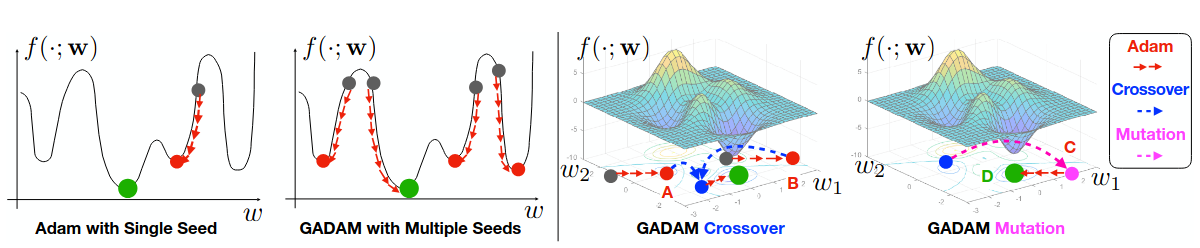
\includegraphics[width=1\textwidth]{img/GADAM.png}
    \caption{Funzionamento di GADAM. Immagine tratta da \cite{gadam2018}}
    \label{fig:GADAM}
\end{figure}
    